%%%%%%%%%%%%%%%%%%%%%%%%%%%%%%%%%%%%%%%%%%%%%%%%%%%%%%%%%%%%%%%%%%%%%%%%%%%%%%%%
%2345678901234567890123456789012345678901234567890123456789012345678901234567890
%        1         2         3         4         5         6         7         8

\documentclass[letterpaper, 11 pt, onecolumn]{article}

\linespread{0.98}
\usepackage{tgpagella}
\usepackage{url}
\usepackage{hyperref}

\usepackage[dvips]{color}

\usepackage{pslatex}
% \usepackage{nopageno}
\usepackage{enumitem}
\setlist{itemsep=0em, topsep=0em}
\usepackage[left=1in,right=1in,top=1in,bottom=1in]{geometry}

\usepackage{tabularx}
%\usepackage{hangcaption}
\usepackage[font=footnotesize]{caption}
\usepackage[final]{graphicx}
%\DeclareGraphicsExtensions{.eps,.ps,.PS,.EPS}
\usepackage{epsfig}
%\usepackage{subfig}
\usepackage{tikz}

\usepackage{amsmath}
\usepackage{amssymb}
\usepackage{fancyhdr}
\usepackage{tikz}
\usetikzlibrary{automata,positioning}

%\usepackage{xspace}
\usepackage{cite}
\usepackage{url}
\usepackage[letterpaper]{}
\usepackage{epstopdf}
\usepackage{authblk}
\usepackage{lineno}
\usepackage{todonotes}
\usepackage{soul}
\usepackage[utf8]{inputenc}
\usepackage[english]{babel}
%\usepackage[font=footnotesize,labelfont=bf]{caption}
\usepackage[font=small,labelfont=bf]{caption}
\usepackage{pgfgantt}
\usepackage[numbers,sort&compress]{natbib}

\usepackage[compact]{titlesec}
\usepackage{subcaption}

\usepackage{titling}
\setlength{\droptitle}{-5em}   % This is your set screw
\setlength{\belowcaptionskip}{-10pt}
\usepackage{titlesec}
\titlespacing*{\section}{0pt}{0.4\baselineskip}{0.4\baselineskip}
\titlespacing*{\subsection}{0pt}{0.4\baselineskip}{0.4\baselineskip}
\titlespacing*{\subsubsection}{0pt}{0.4\baselineskip}{0.4\baselineskip}
\setlist[itemize]{leftmargin=*}

\setcounter{topnumber}{2}
\setcounter{bottomnumber}{2}
\setcounter{totalnumber}{4}
\renewcommand{\topfraction}{0.85}
\renewcommand{\bottomfraction}{0.85}
\renewcommand{\textfraction}{0.15}
\renewcommand{\floatpagefraction}{0.8}
\renewcommand{\textfraction}{0.1}
\setlength{\floatsep}{5pt plus 2pt minus 2pt}
\setlength{\textfloatsep}{5pt plus 2pt minus 2pt}
\setlength{\intextsep}{5pt plus 2pt minus 2pt}

% for comments
\newcommand{\zhi}[1]{\textcolor{blue}{ZL: #1}}
\newcommand{\kris}[1]{\textcolor{green}{JR: #1}}
\newcommand{\jacob}[1]{\textcolor{magenta}{KH: #1}}
\newcommand{\jeanine}[1]{\textcolor{red}{JS: #1}}



% \setlist[enumerate]{leftmargin=*}

\titlespacing{\paragraph}{%
  0pt}{%              left margin
  0\baselineskip}{% space before (vertical)
  0.3em}%               space after (horizontal)

\titlespacing{\subsection}{%
  0em}{%              left margin
  0.15\baselineskip}{% space before (vertical)
  0.15\baselineskip}%               space after (horizontal)

% figures with text wrapped around
\usepackage{wrapfig}
\usepackage{titling}
\setlength{\droptitle}{-5em}   % This is your set screw
\setlength{\textfloatsep}{0.8\baselineskip plus 0.2\baselineskip minus 0.5\baselineskip}

\newcommand{\fig}[1]{Fig.~\ref{#1}}
\newcommand{\figs}[2]{Fig.~\ref{#1} to~\ref{#2}\xspace}
\newcommand{\figa}[2]{Fig.~\ref{#1} and~\ref{#2}\xspace}
\newcommand{\eq}[1]{Eq.~(\ref{#1})}
\newcommand{\eqs}[2]{Equations~(\ref{#1}) to~(\ref{#2})}
\newcommand{\eqa}[2]{Equations~(\ref{#1}) and~(\ref{#2})}

\pagestyle{plain}                                                      %%
%%%%%%%%%% EXACT 1in MARGINS %%%%%%%                                   %%
\setlength{\textwidth}{6.5in}     %%                                   %%
\setlength{\oddsidemargin}{0in}   %% (It is recommended that you       %%
\setlength{\evensidemargin}{0in}  %%  not change these parameters,     %%
\setlength{\textheight}{8.5in}    %%  at the risk of having your       %%
\setlength{\topmargin}{0in}       %%  proposal dismissed on the basis  %%
\setlength{\headheight}{0in}      %%  of incorrect formatting!!!)      %%
\setlength{\headsep}{0in}         %%                                   %%
\setlength{\footskip}{.5in}       %%                                   %%
%%%%%%%%%%%%%%%%%%%%%%%%%%%%%%%%%%%%                                   %%
\renewcommand{\refname}{References Cited}                              %%
\bibliographystyle{plain}



\begin{document}


\setcounter{page}{1}
\pagebreak

\begin{center}
	{\Large \bf FW-HTF Theme 2: Shaping the Socioeconomic Impact of Robotics and Autonomy in Healthcare}
\end{center}

\vspace{1 em}

\paragraph*{\Large Project Summary} 
The increasing adoption of robotics in healthcare poses far-reaching questions about how healthcare personnel will adapt to the use of robotic technology, the role of robot autonomy in a sector traditionally resistant to taking the human out of the loop, and how cognitive assistance for robot operators can be engineered to help avoid disparate impacts on the workforce.  This interdisciplinary project aims to address these questions by bringing together experts in medical robotics, psychology, economics, and medicine to study current and experimental robotic technologies for healthcare applications.  Healthcare robots have been adopted at various stages of maturity, ranging from established technologies like surgical robots and telepresence robots for remote consulting, to experimental but promising applications in rehabilitation, nursing, and home care robots.  They have the promise to improve patient outcomes, deliver high-quality care to rural and remote areas, allow workers whose jobs require physical interaction to telecommute, and provide physical assistance to reduce workplace injuries. And yet, there is a gap in understanding the socioeconomic impact of these technologies on patient-caregiver relationships, the job market, training, and job satisfaction of healthcare personnel.  This project hypothesizes that increasing robot adoption runs the risk of disparate impact on certain classes of healthcare worker, including biases from gender, age, and socioeconomic status.  Although the relationship between technology and workforce development is highly complex, the project hypothesizes that a major factor in this relationship is the amount of cognitive assistance provided by the user interface.  Using a mix of economic, psychological, and engineering methodologies, this research seeks to clarify the links between cognitive assistance and socioeconomic impact, and to develop best practices for engineering robot interfaces and worker training programs.

% Tele-operated robotic systems extend a human worker’s physical capabilities to perform manufacturing and maintenance tasks in remote, inaccessible, dangerous and/or hazardous environments. 
%This project aims to (1) develop novel teleoperation interface and training methodology that facilitate healthcare workers to acquire the motor skills of controlling complex motion coordinations frequently performed in nursing and assisting tasks; and (2) investigate the impacts of the proposed technology and training paradigm on healthcare jobs given the socio-cultural norms and biases. The state-of-the-art tele-nursing robots have been endowed with the physical structures for performing arm-hand coordination, bimanual coordination and loco-manipulation while perceiving environment through multi-model sensors from various perspectives. However, these capabilities haven't been exploited due the difficulties of learning the motion and perception mapping imposed by teleoperation interface. Measurement metrics for human and robot performances are not sufficient to quantify the characteristics of teleoperation interfaces, and compare the synergistic human-robot performance through the interfaces across tasks and along the user's motor skills progression. Novel training paradigm to adapt to the technology advancement hasn't been investigated in nursing education. On the social-economical side, it is unclear if the novel tele-nursing technology will significantly shift the job market due to socio-cultural biases (e.g., gender, age, etc) and the correlated education barriers. The socio-cultural biases may interfere with the design of the device and also the desire and ability to learn and use (tele)operation interfaces. For instance, it is possible that during the design process differences between genders are not examined. It is also possible that women are less interested (or even less able) to use (tele)operation interfaces due to gender bias or stereotype threat. Likewise, patients may be less likely to trust a tele-operated robotic system if it controlled by a female compared to a male.  

%To address the above technological, educational and social-economical issues, we propose to synergize research efforts from robotics, nursing education and Social psychology to achieve the following research objectives. Our Science and technology objectives aim to (1) Develop novel metrics to characterize the teleoperation interface (the operation complexity, motion mapping intuitivity, efficiency and predictability, perception transparency and balance, etc., and compare various teleoperation interfaces developed for a mobile humanoid nursing robots in motion coordination tasks. Based on the understanding of human-robot adaption through the teleoperation interfaces, we will further develop technologies that can (2) Shift the boundary between direct teleoperation and autonomous control based on the physical and mental status of the operator, (3) synthesize and convert sensory information to improve cognitive situation-awareness, and improve cognitive and physical skills of the operator, (4) Infer human teleoperator's contextual intent based on the knowledge of manipulation tasks and human motions, in order to automate appropriate low-level robot actions.  Our education objective aims to (1) Integrate ``cloud wisdom'' of multiple intelligence agents (human experts and AIs) into the skill evaluation and collaborative decision-making in terms cognitive augmentation, (2) Utilize interactive perception to engage the learning user to actively explore the robot's motion and perception capabilities. Our social-economy objectives aim to (1) determine nursing tasks where a tele-operated robotic system will be of assistance and design robotic system, (2) investigate perceptions of tele-operated robotic systems in relation to socio-cultural norms and biases to assist in the design and implementation. 

\vspace{0.5 em}

\paragraph*{\Large Intellectual Merit}
The intellectual merit of this proposal is to 1) clarify the connection between robotic technology adoption and socioeconomic impact in a broad range of healthcare sectors, and 2) to understand how cognitive and physical assistance in healthcare robots may impact job satisfaction and mitigate possible disparate impacts.  Moreover, novel technologies for intelligent user interfaces based on machine learning and artificial intelligence will be developed and evaluated on robotic telesurgery, telenursing, and in-home care applications.  Human subjects studies will help better understand how gender bias, stereotype threat, and other socio-cultural norms may be at play in robotics, which will further influence technology development and worker training. 

%This project addresses how multi-modality teleoperation interface affects the adaption of human motor behavior adapt to the motion and perception capabilities of a robotic physical embodiment. It develops novel methodologies to evaluate the adaption level by the quality of low-level motor skills and high-level task plan. It uniquely integrates collaborative skill evaluation method to teleoperation skill acquisition process, and guides the learning process by maximizing the expected perception and motion information gain.  Moreover, this will be some of the first work to explicitly examine the effects that gender has on: a) perceptions of tele-operated robotic systems, individuals desire and ability to use tele-operated systems, and b) perceptions of the competence of the user of the tele-robotic system. It develops a unified framework that takes into consideration gender bias, stereotype threat, and other socio-cultural norms that may be at play, which will further influence the technology development and worker education. 

\vspace{0.5 em}

\paragraph*{\Large Broader Impacts}
This research will have the broader social impact of benefiting healthcare workers that operate or will operate robots in the course of their job duties, as well as other job sectors that are beginning to see workers interact with robots, like autonomous driving, manufacturing, agriculture, and household robots. The adoption of robots into these sectors can reduce the exposure of human personnel to dirty, dull, and dangerous tasks, and reduce the ergonomic and physical demands of certain tasks that have disparate impact on women and the elderly.  Research will be closely linked to graduate and undergraduate education for students from engineering, social sciences, and medical schools, and outreach to K-12 students and the general public will also be pursued. 

\pagebreak

\pagebreak

% \maketitle

\vspace{-4pt}

\pagestyle{plain}
\setcounter{page}{1}


\setcounter{page}{1}

%-------------------------------------------------------------------------
\section{Introduction and Significance}\label{sec:intro}
%-------------------------------------------------------------------------

Major challenges facing the healthcare system in the US and worldwide include an aging population, high costs of treatment, increasing clerical burdens, and a shortage of doctors and nurses. These problems call for forward-thinking socio-technological solutions, and one approach currently being considered is to adopt robotics into various aspects of healthcare.  Robots have the potential to dramatically change the practice of clinical care in the near future as hospitals begin to adopt surgical robots to enhance surgeon dexterity in minimally invasive procedures, telepresence robots used for remote consultation, food and medicine delivery robots, assistive robots for elder care, patient lifting robots, and teleoperated robots for clinical care in quarantine rooms.  However, the socioeconomic implications of robot adoption on the state of patient care and the healthcare workforce are still poorly understood.  From the point of view of patients and caregivers, the use of robotics to augment or replace job responsibilities may be considered to be hostile, degrading, and even discriminatory. At these early stages of technology development, the time is ripe to carefully consider these implications so that their positive and negative consequences can be better predicted and hopefully controlled to preserve broad access to productive and meaningful work.

The purpose of this project is to investigate two general thematic questions regarding the adoption of robotics in healthcare.  First, how can cognitive assistance in these robots, in the form of autonomy or partial autonomy, be designed to satisfy workers' occupational needs while maintaining adequate technical performance?   Second, how will the increasing adoption of robots  potentially benefit or harm healthcare workers and the broader healthcare system?   These themes are {\em multifaceted}, involving engineering, psychological, and socioeconomic issues, and they are {\em overlapping}, since the nature of cognitive assistance provided by the human interface will inevitably affect how workers adapt to robotic technology.  This three-year collaborative research project assembles an interdisciplinary team to address these questions using methodologies from economics, psychology, and engineering.  Although this project is focused on the context of healthcare, the results from this research will also be relevant to broader questions of embodied intelligent cognitive assistants at large.

To address these questions, the activities of this project are organized along three specific aims:

\begin{itemize}
\item \textbf{Aim 1: Develop frameworks for autonomous cognitive assistance in healthcare robots} --- Evaluate forms of cognitive assistance across a range of healthcare robots.  Study information displays for complex, multimodal sensor information and background knowledge.  Implement partially automated tasks that may be routine, difficult for direct control, or cooperative with humans.  Investigate algorithms for inferring human operator intent for coordination with humans, and adaptive task scheduling for cooperative human-robot teams.

\item \textbf{Aim 2: Model the socioeconomic impact of healthcare robots} --- Study the impact of robotic adoption on the economy and labor market.  Survey healthcare worker attitudes toward robotics and study the robot training process for telerobotic (non-autonomous) systems.  Characterize potential disparate impacts by location, gender, race, and age. 

\item \textbf{Aim 3: Model the interaction between autonomy and impact} --- Study human factors issues regarding the human-autonomy interface.  Characterize how autonomous features of healthcare robots may affect disparate impacts, and suggest best practices for future technology development.

%\item \textbf{Aim 1, Technology} ---  Study the Developed Motion-Perception Coordination: Compare developed teleoperated motion coordination across various teleoperation interfaces; Investigate the motion coordination strategy under passive, active, and interactive perception; Study the regularity and variability of the developed motion coordination across teleoperation interfaces, to reveal the adaption of human motor control to robot motion and perception capabilities. 

%\item \textbf{Aim 2, Education} --- Study the Motion Coordination Development Process: Develop performance evaluation metrics for human-robot teleoperation system; Study the progression of teleoperated motion coordination from novice to expert, and identify the milestones and thresholds of performance improvement; Investigate the evolution of motion primitives and task plan; Prescribe multi-modality cognitive augmentation to overcome the skill development thresholds; Prescribe physical-cognitive training tasks to develop transferable skills for perception-motion coordination. 

%\item \textbf{Aim 3, Social-economy} --- Compare the skill development processes among populations different in gender, race, and age; Evaluate the potential effects of cognitive function differences and socio-cultural biases on robot teleoperation skill acquisition. 

%\item \textbf{Aim 4} --- Integrate Aim 1-3; Develop novel teleoperation interfaces that can (1) support transparent and intuitive human-robot adaption, (2) convey to teleoperator most concise and relevant performance indices and task information to facilitate task development, (3) evaluate novel teleoperation skill training paradigm across different populations. 

\end{itemize}

The team has a unique capability to use experimental robotic testbeds for this research in the areas of {\em telesurgery}, {\em telenursing}, {\em rehabilitation}, and {\em in-home care}.  Although there are other forms of robotics being adopted in healthcare, these testbeds represent different points along the spectrum between existing (telesurgery, telemedicine) and promising future technologies (rehabilitation, telesurgery, in-home care).  Moreover, the endpoints of this spectrum roughly correspond to tele-robotics vs autonomous robots.  While existing surgical robots are directly operated by surgeons, in the near future, healthcare personnel will be operating robots at various levels of autonomy, ranging from direct teleoperation (no autonomy) to supervisory control (all low-level motor functions autonomous). Tele-robotic systems enable medical workers to perform surgical, nursing, assisting and rehabilitation tasks in remote, inaccessible, and/or quarantine environments. Through tele-robotic technologies, single operator can operate multiple robotic systems (fan-out), and rapid switching between robots dispatched to different service sites. On the other hand, autonomy provides cognitive assistance that aims to reduce the cognitive burden on a human operator, allowing them to focus on other tasks or to operate multiple robots. Increased automation leaves the human operator in the role of decision-maker rather than a pilot, which may make the job less tedious or more interesting. Automating the “dirty” parts of a job, or reducing the time spent in clerical work, could also lead to higher job satisfaction.  However, the use of autonomy faces resistance in the healthcare sector, which prefers to keep doctors and nurses in control of decision-making.

Although the relation between technology use and job satisfaction is complex, it can be reasonably hypothesized that technology is becoming a larger part of a worker’s job, their job satisfaction will be less negatively affected if the technology is more transparent or a worker is more comfortable with it. The ultimate study in this proposal (Aim 3) will be aimed at assessing whether healthcare robots that employ cognitive assistance for the operator will be viewed as more transparent and accepted by healthcare workers. These attitudes will be assessed with medical personnel and students across gender, age, and socioeconomic factors.

%From a novice to an expert teleoperator, human workers learn to adapt their motor control to the motion and perception capabilities of the robotic physical embodiments of their remote surrogates. 



% To reduce the workers' skill acquisition efforts, we propose to compare the motion coordination teleoperated through various interfaces, by users of developed and developing teleoperation skills. We investigate the regularity and variability of the developed motion coordinations across teleoperation interfaces, to reveal the underlying strategies of natural human motion and perception coordination. We also compare the developing motion coordinations during the training, to identify the milestones and threshold of the teleoperation skill progression.   


% in their , 

% our project will investigate the underlying strategies of natural human motion and perception coordination, and develop teleoperation interfaces that support intuitive perception and motion mapping.   


\paragraph*{Intellectual Merit.}
This research will investigate \textbf{novel user interfaces} that can fully synergize human and medical robots' physical and cognitive capabilities, \textbf{novel training paradigms} that can help medical personnel learn to use robots effectively, and \textbf{an enhanced understanding of socio-cultural norms and biases} in medical training and practice. 

\paragraph*{Broader Impacts.}  The outcomes from this research will help predict the potential impact of robotic technologies on healthcare jobs, and reduce bias based on location, gender, race, and age.

\paragraph*{Qualification of Investigators.}
The engineering team has extensive experience in robotics, and have developed robots for tele-surgery, rehabilitation, tele-nursing, and home care. The social science team consists of experts in gender bias, human factors, surgery, and nursing, including cross-disciplinary expertise in the implementation of autonomous interfaces and telemedicine. Robot platforms available for use in this research, built and operated by the co-PIs in prior work, include the Raven telesurgical robot, [WHAT REHABILITATION ROBOT], and two TRINA mobile manipulators. 

% Tele-robotic systems extend a medical worker's motion and perception capabilities to perform surgical, nursing, and rehabilitation tasks in remote, inaccessible, and/or hazardous environments. These tasks are risk-sensitive tasks usually involve intimate interaction with patients, and thus far can only be accomplished under direct teleoperation instead of autonomous control. Task performance heavily depends on the the human teleoperator's dexterous motion coordination skills, developed situational awareness, and domain knowledge for decision-making and situation evaluation. The state-of-the-arts medical robotic systems have been endowed with complex and capable motion and perception hardwares. The physical capabilities of medical robots and human teleoperators are bottlenecked by low-transparency teleoperation interfaces. To freely and efficiently control their remote surrogates, human workers need to devote significant efforts to learn the motion and perception mapping defined by the teleoperation interface. To address these needs, we propose to investigate motion/perception mapping , and develop a user interface to support intuitive robot control and multi-modality cognitive augmentation. 

% Our proposed project aims to (a) reduce the teleoperation control effort in dexterous and coordinated manipulation tasks, (b) facilitate novice workers to acquire the fine motor skills for operating complicate robotic systems to work on various manufacturing tasks, (c) propose novel worker training infrastructure and methodologies improve the skills and well-being of industrial workers, and (d) create safe, comfortable, and remotely accessible industrial job opportunities. We propose research objectives with the emphases on \textit{science and technology}, as well as \textit{education and social-economy}. Our Science and technology objectives aim to investigate theories and technologies that (1) Shift the boundary between direct teleoperation and autonomous control based on the physical and mental status of the operator, (2) synthesize and convert sensory information to improve cognitive situation-awareness, and improve cognitive and physical skills of the operator, (3) Infer human teleoperator's contextual intent based on the knowledge of manipulation tasks and human motions, in order to automate appropriate low-level robot actions. Our education and social-economy objective aims to (1) Integrate ``cloud wisdom'' in terms cognitive augmentation into the collaborative decision-making and motor learning process among multiple intelligence agents (human experts and AIs) through a democratic or weighted voting system, (2) Study the effect of cognitive-augmentation human-robot interface on industrial worker skill acquisition and mental/physical demands in training processes, (3) Develop novel training methodologies and infrastructure at home and in workplace, and (4) Investigate the social-economical impacts of such technology on small and large industries, and on societal job opportunity shift and regional and national job distribution.  


\paragraph*{Relevance to the goals of NSF's FW-HTF Big Idea}

\textcolor{red}{(a) transforming the frontiers of science and technology for human performance augmentation and workplace skill acquisition; (b) improving both worker quality of life and employer financial metrics; (c) enhancing the economic and social well-being of the country; and (d) addressing societal needs through research on learning and instruction in the context of augmentation.}


This will be the first work to explicitly examine the effects of age, gender, and socioeconomic status on: a) attitudes and acceptance of healthcare robot operation as part of job responsibilities, b) perceptions of one's own competence when operating a robot, and c) attitudes and acceptance of cognitive assistance provided by semi-autonomous interfaces.  The resulting theories of gender bias, stereotype threat, and other socio-cultural norms that may be at play, will inform the future of technology development and worker training. 
 
\paragraph*{Vision of success for the proposal}
\textcolor{red}{Specifically define the project goals and the definition of a successful outcome.}

Specific goals for the project include: 1) conduct an economic analysis of the impact of robotics on the healthcare labor market and healthcare industry, 2) survey the attitudes of nurses and doctors toward the use of robots as a conduit for or replacement for job responsibilities, 3) develop autonomous functions for tele-surgical and tele-nursing robots including at least one routine task and at least one difficult task, 4) conduct human subjects studies to understand worker attitudes toward shared control or semi-autonomous functions, 5) characterize how cognitive assistance in healthcare robots may affect disparate impact, and 6) suggest best practices for future robotic technology development.
\section{Background and Related Work}

\subsection{Intelligent task automation for medical worker capability augmentation}

Similar to the industrial revolution, task automation has been transforming the interaction and collaboration of human workers and AI agents in healthcare, industry, social service and military tasks. This ``white-collar revolution`` has significantly changed the paradigm of human-robot teleoperation. On one hand, intelligent assistive robots augment the physical and cognitive capabilities of human workers, relieve them from repetitive, tedious, effort-demanding, and dangerous tasks. On the other hand, the-state-of-the-art intelligent robot cannot perform complex and risk-sensitive task without human control. As the tasks for robots increasing with the robot capabilities, teleoperation, with more or less task automation, will remain to be the most reliable way to perform the most difficult tasks. It is also the most efficient way to synergize human-robot performance, and explore and utilize robot physical capability.
In this context, physical and cognitive augmentation, in terms of automated information system and automated motion control system,  becomes a necessary components to various medical robotic system. Medical robotic systems have been equipped with various level of intelligent assistance that automate tasks hard or tedious for direct human control. Robot motion planning and learning has enabled the automation the pre-defined motion coordination in rehabilitation and simple, routine surgery procedures.  For more free-style tasks, robot teleoperators have been assisted with motion smoothing and scaling for improved precision control, and with power augmentation in labor-demanding work. However,  due to the little knowledge of task structure and user intent, robots are not clear about which part of the task can be automated and have to depend on teleoperators to micromanage its motion coordination. Conventional interfaces tend to limit the degrees of freedom that human can control directly and/or simultaneously. These interfaces reduce human control efforts, yet impose unnecessary constraints to the motion coordination robot can perform. Novel teleoperation interfaces control map natural human motion using motion capture systems, wearable sensors and exoskeletons, yet the difference in human and robot embodiments usually prevent straightforward motion mapping.  In addition to demanding mental efforts for robot motion control, medical workers can also be limited in or overwhelmed by task information.  Teleoperation interfaces cannot identify the task-relevant perception and performance information, and present in the way comfortable for human to process. The technology limitation compounds the socio-cultural bias in gender, age, and socioeconomic status, prevents the synergy of medical workers and robotic technology.  

\subsection{Prior work in the literature}


Robots have the potential to help distribute expertise around long distances using tele-robotics, to reduce costs by automating routine tasks, and protect workers against occupational hazards and ergonomic strain.  These potential benefits are already being adopted into healthcare.

\textcolor{red}{TODO: need references on gender and age bias with technology.  Needed from Jeanine}

\textcolor{red}{TODO: need references on economic impact of robotics and automation.  Needed from Alex}

\textcolor{red}{TODO: clean up and add references to telerobotics and autonomy}
Collaboration between humans and autonomous robotic agents has the potential to improve safety and efficiency across a wide range of industrial settings, including manufacturing, medicine, maintenance, and construction (Fong, Thorpe, \& Baur, 2001; Tan, Duan, Zhang, Kato, \& Arai, 2009; Kock, et al., 2011; McDonald, Small, Graves, \& Cannon, 1997). An important set of challenges in the design and implementation of human-autonomy collaborative systems is developing a clear understanding of the task environment and potential agent roles, the interdependencies between human and robotic agents, and the impact of disruptions (e.g. (Tan, Duan, Kato, \& Arai, 2010; Hoffman \& Breazeal, 2004; Drury, Scholtz, \& Yanco, 2003; Mutlu, Osman, Forlizzi, Hodgins, \& Kiesler, 2006)).

Managing the safety and efficiency of such systems under dynamic settings is particularly challenging given the complexities of such work environments. For example, a response to a dynamic failure (such as a human or robot breakdown) will have different considerations dependent upon the work architecture (the functional allocation between robots and human) and nature of the work environment (structured vs. unstructured, e.g. (Kolski, Ferguson, Bellino, \& Siegwart, 2006; Scholtz, 2003)). How to effectively optimize safety and efficiency, which are often competing variables, and dynamically reallocate resources accordingly creates a challenging problem for managers and schedulers of such complex systems.

Management of worker and equipment scheduling, coordinating equipment maintenance, tracking of production and safety metrics and ensuring appropriate quality control are all key considerations for supervisors of modern manufacturing environments (e.g. (Brumson, 2008; Brandimarte, 1999)). The challenges associated with managing all of these factors are made more complex by the introduction of collaborative human and robotic work environments, which is a nascent interdisciplinary field. In current manufacturing environments humans and robots work in zones of exclusivity, both physically and for task assignments (Krüger, Lien, \& Verl, 2009; Fryman, 2014; Unhelkar \& Shah, 2015). However, with the emergence of robots that can work alongside humans, like the Baxter™ robot (Figure 1), soon human-robot teams  that jointly work on tasks will be commonplace. 


The increased capabilities that collaborative human-robot teams will bring also introduce complexities in scheduling activities, particularly under dynamic replanning conditions  that occur when both humans and robots “malfunction”, i.e., humans call in sick at the last minute or robots unexpectedly stop working (Wilcox, Nikolaidis, \& Shah, 2013; Stubbs, Wettergreen, \& Hinds, 2007). The impact of these contingencies on the productivity of a manufacturing line will depend upon the nature of the task, the architecture of the work environment, and the availability of substitute workers (either human or robot). The flexibility of the work architecture will dictate the options with which a scheduler or manager can shift assets to minimize the impact on production when problems arise. Indeed, even in current manufacturing operations, such last-minute, dynamic replanning scenarios are difficult to manage even without the added complexity of jointly-tasked human-robot teams (Leitão \& Restivo, 2008). In collaborative human-autonomy environments, addressing such dynamic replanning conditions will be even more challenging, and an inefficient decision could result in a significant decrement in production or increase in safety risk.

There is a long history of research on the incorporation of robotic agents in manufacturing systems (Hägele, Nilsson, \& Pires, 2008; Krüger, Lien, \& Verl, 2009). Typically, these efforts have focused on the use of physical or temporal separation from humans to ensure safety (Marvel \& Bostelman, 2013; Fryman, 2014; Unhelkar \& Shah, 2015; Tan, Duan, Zhang, Kato, \& Arai, 2009; Eilering, Franchi, \& Hauser, 2014). More recently, there has been interest in the inclusion of robotic systems in manufacturing environments that require close interaction and collaboration of human and robotic agents (Office of the Secretary of Defense, 2013; Ryan \& Cummings, 2014; Scanlon, 2009; Rio Tinto, 2014) (Nikolaidis, Ramakrishnan, Gu, \& Shah, 2015). Most of the prior research on human-robot collaboration has focused on the localized methods of interaction and communication of commands and intent between a human worker and a robotic worker (Gombolay, Huang, \& Shah, 2015; Inagaki, Sugie, Aisu, Ono, \& Unemi, 1995; Green, 2008; Bauer, Wollherr, \& Buss, 2008; Fernandez, Balaguer, Blanco, \& Salichs, 2001; Li \& Hauser, 2015; Hoffman, 2013). For example, Fernandez et al. (2001) experimented with determining intent of humans in a collaborative carrying task based on the force signal measured in the arm gripper. Maintaining safety in such collaborative environments has also continued to be an active area of research (Tan \& Arai, 2011; Fryman, 2014; Pedrocchi, Vicentini, Matteo, \& Tosatti, 2013; Matthias, et al., 2011). However, there is very little research on more global interactions of humans and robots in terms of developing integrated schedules, and how such interactions drive large productivity and safety goals.

Traditionally, scheduling of robotic systems have focused on artificial intelligence (AI) or rule-based scheduling (e.g. (Miyashita, 1998; Hall, Kamoun, \& Sriskandarajah, 1998; Sikora \& Shaw, 1997)), though have acknowledged the usefulness of including a human supervisor in the scheduling process (Chen \& Guerrero, 1992). It has been demonstrated that human supervisors can improve scheduling decision-making through the coaching of automated systems, e.g. (Barnes, Chen, Jentsch, \& Redden, 2011; Cummings, Brzezinski, \& Lee, 2007; Adams, 2009; Chen \& Barnes, 2012; Fagerholt, 2004; Törnquist, 2006). While these studies have shown the benefit of automation-aided decision making, these environments generally considered automation in terms of “expert” systems, which operate deterministically by pre-programmed rules. What they have not addressed is the task dependencies and scheduling challenges associated with proposed human-autonomy collaborative manufacturing environments, which contain significant uncertainty and many more stochastic variables.

Still a relatively new field, current research into task scheduling for robotic and collaborative environments focuses on detailed elements of timing and motion constraints (e.g. (Gombolay, Wilcox, \& Shah, 2013; Shah, Conrad, \& Williams, 2009; Boerkoel Jr \& Durfee, 2011; Gowal \& Martinoli, 2012), but does not address higher level considerations such as short and long term impacts to higher level global considerations including overall schedule, throughput, maintenance scheduling, and ergonomic risk. The proposed work aims to fill these gaps by investigating decision-support tools for collaborative manufacturing environments that incorporates both short and long term, and local and global implications of current and proposed schedules.

\subsection{Socio-economic bias in the usage of intelligent medical task automation}

Intelligent task automation aims to improve the availability of high-quality healthcare service while reducing the cost.  It also aims to reduce the control and learning efforts in the usage of healthcare robots, equalize worker performance, lower the barrier to healthcare professions, and improve job satisfaction of medical workers. Despite the good intention of technology development,  the potential psychological and socioeconomic implications needs to be fully understood to evaluate the socioeconomic impacts that may be brought by the usage healthcare robots. 
One issue that needs to be investigated with healthcare robots is the issue of bias.  Bias can come into play in many different forms within health care.  One way in which bias can come into play is through health care workers (i.e., physicians or nurses), Healthcare workers are not immune to bias and use implicit bias related to race, gender, and culture when treating and making decisions about patients (Chapman, Kaatz, \& Carnes, 2013; Taylor, 2003; van Ryn \& Burke, 2000).  Healthcare workers also have preconceived notions of robotic devices and unless they seem easy to use or useful are unlikely to be adopted (BenMessaoud, Kharrazi, \& MacDorman, 2011).  Thus, it is important to understand if assistive robotic technologies can help mitigate this biases or if they will exacerbate them.  
Another way in which bias plays a role in healthcare is through the patients themselves.  Patients experiences with healthcare workers influences their satisfaction with their care, and research has found that female and minority patients are less satisfied with physician and nursing care than male and white patients (Blendon, Scheck, Donelan, et al., 1995; Cooper-Patrick, Gallo, Gonzales, et al., 1999; Foss, 2001; Saha, Komaromy, Koepsell, \& Bindman, 1999).  Minority patients also feel as if they are treated differently and more unfairly than white patients by healthcare workers (Johnson, Saha, Arbelaez, Beach, \& Cooper, 2004).   Thus, it is important to examine how women and minority patients feel about assistive robotic technologies and how they impact their perceptions of the quality of care.  It is possible assistive robotic technologies will be well received as they are receiving high-tech assistance, but it is also possible that assistive robotic technologies will increase feelings of poorer care as it may limit human-to-human interactions between patients and their healthcare providers.  


Another area where bias can come into play is the design of the assistive robotic technologies.  There is already evidence that gender and racial stereotypes emerge in technologies.  For instance, gender stereotypes are often perpetuated in technologies and AI devices because women are often not included in test populations or thought of during the design process (Oost, 2003; Oudshoorn, 2003).  One example of this is that voice recognition systems have a harder time detecting female voices compared to male voices and this included medical voice dictation software (Carty, 2011; Rodger \& Pendharkar, 2004; Taman, 2016).  In addition, women searching for jobs were shown different, and lower paying, search results than men searching for jobs using the same terms (Howard \& Borenstein, 2017).  It is even argued that technological advances help maintain gender biases in society and maintain the status quo (Kilbourne \& Weeks, 1997).  Racial stereotypes are also prevalent in technologies and AI as well (Howard \& Borenstein, 2017).  For instance, Google’s mobile photo app labeled black individuals “gorillas” (Pulliam-Moore, 2015) and image searches for “black teenagers” was more likely to bring up images of criminal activity than a search for “white teenagers” (Howard \& Borenstein, 2017).   Thus, it is important during the design phase of the assistive technologies that measures are taken to ensure the devices limit the proliferation of biases (Howard \& Borenstein, 2017).  

\subsection{Related work of the investigators}

% \begin{wrapfigure}{r}{0.75\linewidth}
\begin{figure}[h!!]
\centering
% \vspace{0.8ex}
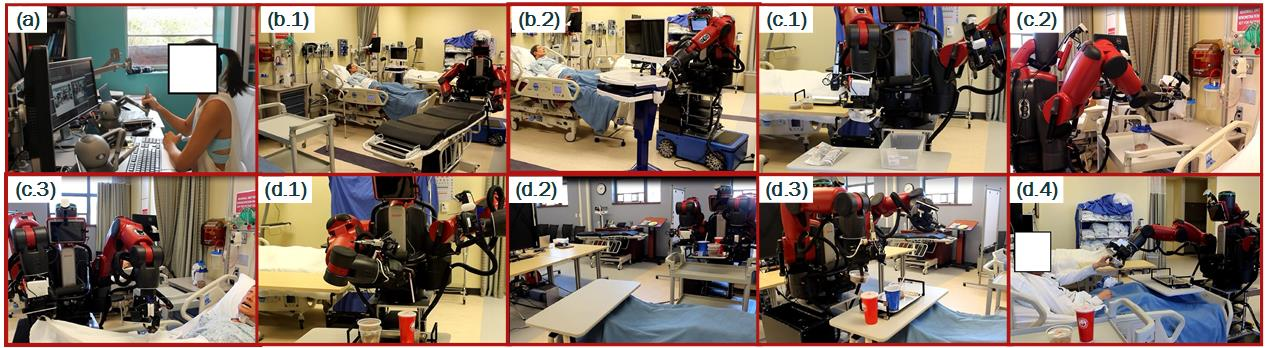
\includegraphics[width=0.99\linewidth]{fig//NursingTask}
\caption{Under (a) direct teleoperation, a mobile humanoid robot tasks can perform complex nursing tasks, including (b.1-2) moving a portable medical devices; (c.1-3) organizing and cleaning the patient's room; and (d.1-4) preparing and serving food to a patient. These tasks involves the coordination among multiple robot components for manipulation, locomotion and active perception.}
\label{NursingTask}
\vspace{1ex}
\end{figure}
% \end{wrapfigure}

\begin{itemize}
\item \textbf{Tele-nursing Robots} In response to the outbreak of highly infectious diseases, including Ebola (2015) and Zika (2016), Tele-Robotic Intelligent Nursing Assistant (TRINA) --- a tele-presence-tele-action mobile humanoid robot system --- has been developed and over frequently performed nursing tasks (see~\fig{NursingTask}). The nursing robot is equipped with fixed cameras mounted at the head and chest, and moving cameras attached to the wrists. Thus, a teleoperator is able to control the coordination of the robot's perception and action arms, in addition to the coordination of different robot components (e.g., arms, hands, mobile base). The experimental system evaluation has demonstrated that on average the tele-nursing robotic system controlled by expert teleoperator is 95X slower than expert human nurse. This performance can be significantly improved by developing a teleoperation interface of more transparent perception and motion mapping. 

\zhi{Figures for tele-surgery tasks to be added}

\item \textbf{Tele-surgical Robots} Surgical procedures are traditionally performed by two or more surgeons along with staff nurses: one serves as the primary surgeon and the other as his/her assistant. Raven IV, a compact multi-arm surgical robotic system, has been developed to enable the collaboration in surgery operation. By automating frequently performed surgical procedures, including dissection, suturing, and tissue manipulation, surgeons can be relieved of the cognitive burden of controlling direct operation and thus focus surgery decision-making. Tele-surgical robot interfaces can further augment a surgeon's cognitive capabilities by integrating ``cloud wisdom'' --- a collaborative decision-making ensemble of multiple intelligence agents, including human experts and AIs. \textcolor{red}{TODO: need details from Jacob.}

% While low-level task automation cognitive augmentation 
% Introducing surgical robots into the operating room has significantly changed the dynamics of interaction between the surgeons and with the surgical site. Through surgical procedure automation, surgical robots relieve the 

% it is  challenging  for  the  surgeon  to  estimate  distances  and
% angles  through  an  endoscope.  Additionally,  with  limited
% vision and/or haptic feedback, extracting the needle from the
% desired  point  often  requires  multiple  attempts,  resulting  in
% increased tissue trauma and extended operation time


% In robot-assisted minimally invasive surgery, a surgeon needs to control the motion of surgical robot arms while adjusting the endoscopic camera to perceive the surgical site. The motion coordination become more complicated when multiple surgical instruments are operating in the shared workspace. The endoscopic camera needs to appropriately with respect to the operating surgical tools, so that the surgeon can intuitively and correctly perceive the spatial relationship at the operation site. The teleoperation interfaces also need to inform the surgeons of their task performance and the patient vital signs, to assist their operation and decision-making.

\item \textbf{Exoskeleton for stroke rehabilitation}
Stroke recovery benefits from intensive and engaged exercises under the direction and assistance of therapists. In stroke rehabilitation, a dual-arm upper limb exoskeleton (e.g., EXO-UL7, see Figure) can assist patient motion during repetitive tasks, provide accurate real-time physical and physiological measurements, promote recovery by coupling the motion of stroke-impacted and healthy arm, and integrate virtual reality games to improve patient engagement and motion-perception coordination. To therapists, the rich measurement information and rehabilitation task prescription parameters cannot be harnessed without cognitive assistance that automates the detection of voluntary motion intent and the evaluation of patient motor performance. Patients also need to be informed of and engaged by feedback on their practice result and performance, to make conscious efforts towards recovery. 

\item \textbf{Hospital administration} The challenges in hospital administration are compounded by significant scheduling uncertainties such as unplanned absences by workers, equipment breakdowns, or worker injuries. The ability of supervisors and management to dynamically adapt role assignments and schedules (what we term as dynamic replanning) is important for dealing with these uncertainties and maintaining adequate patient care. Our prior work has included the preliminary design of a decision support tool for scheduling human shifts in manufacturing environments (Malik, 2013) (Figure 4). This tool allows a supervisor to view the current schedule in the context of required skills and individual ergonomic risk. 

\textcolor{red}{TODO: add prior related work in gender bias, economics, etc.  Needed from Jeanine, Alex}
% \zhi{Figures for tele-rehabilitation tasks to be added}

% \item \textbf{Tele-rehabilitation Robots} Tele-rehabilitation exoskeletons enable therapists to guide and assist remote patients with power augmentation  


\end{itemize}
\pagebreak

%-------------------------------------------------------------------------
\section{Research Plan}\label{sec:plan}
%-------------------------------------------------------------------------
\textcolor{red}{TODO: Jane: outline the approach taken by the team.}

%-------------------------------------------------------------------------
\subsection{Specific Aim 1: Develop frameworks for autonomous cognitive assistance in healthcare robots}\label{sec:plan-task1}
%-------------------------------------------------------------------------

\subsubsection{Automation of routine skills}
\textcolor{red}{TODO: Kris, Jacob}

This Task aims to develop an extensible foundation of hardware capabilities and reliable primitive skills that are applicable for the clinical domain.  We shall identify high-priority capabilities needed for a nursing robot.  Based on prior testing, we have already identified navigation, pick-and-place,
button-pressing, and surface cleaning as key tasks to be implemented.

Via  an  NSF  RAPID  Ebola  seed  grant,  the  Duke  team  developed  the  TRINA
platform (Figure 1) with the goal of enabling nurses and other workers to perform routine diagnostics and
care to infectious patients (i.e., Tuberculosis, Ebola, SARS, etc.) with zero personal exposure to pathogens. From a safe location, a human nurse can log on to TRINA to communicate with patients and other workers
via audio/video communication, navigate around obstacles, measure vital signs, bring food and medicine,
operate equipment, and move carts and furniture.

\paragraph{Primitive Skill Definition.} 
 By a primitive skill we refer to a finite-duration procedure that controls the low-level behavior of the robot in response to requested {\em skill parameters} and the {\em context} of the robot/environment state.  A skill has the following properties:
\begin{enumerate}
\item {\em A precondition} that dictates when it can potentially be applied.
\item {\em One or more postconditions} that may result, including correct operation (e.g., picking up requested item), incorrect operation (e.g., object cannot be picked up), or unexpected errors (e.g., object fell).
\item {\em Probability distribution over postconditions}.  These will be seeded with an unconditional distribution, and their conditional dependence on skill parameters and context will be learned over time through experience~\cite{Pasula_learningprobabilistic2004}.
\item {\em Real-time status information} may optionally be fed back to a human operator.
\item {\em Can be interruptable} or have skill parameters changed during execution.
\end{enumerate}  

Following~\cite{HauserTAMP2010}, the skill parameters may be either continuous or discrete variables.  Examples of continuous variables include target position for a navigation skill, a target object pose for a pick-and-place skill, or an area for a cleaning skill.  Discrete variables may include arm choice, object name, target location name, or button name.  Semantically specified discrete variables will index into a {\em knowledge base} that contains geometric models, physical information, and other properties of known objects, places, and robot poses.

\paragraph{2D Navigation.}  We use laser sensors and the Google Cartographer package to maintain 2D maps of the hospital floor. We have demonstrated collision-free omnidirectional navigation in the robot's local neighborhood.  We will extend this work to optimized  longer-term trajectories, as well as to named places.

\paragraph{Button pressing.} Buttons, knobs, and switches are ubiquitous in clinical environments.  In fact, nurses that we consulted during the development of TRINA 1.0 remarked that turning off alarms would be one of the most useful functions of the robot, since false alarms are frequent, irritating, and a waste of time, especially in quarantine environments in which PPE must be donned and doffed. Button pressing requires relatively precise maneuvering and force application, and hence teleoperation is relatively slow for this skill.

\begin{figure}
\centering
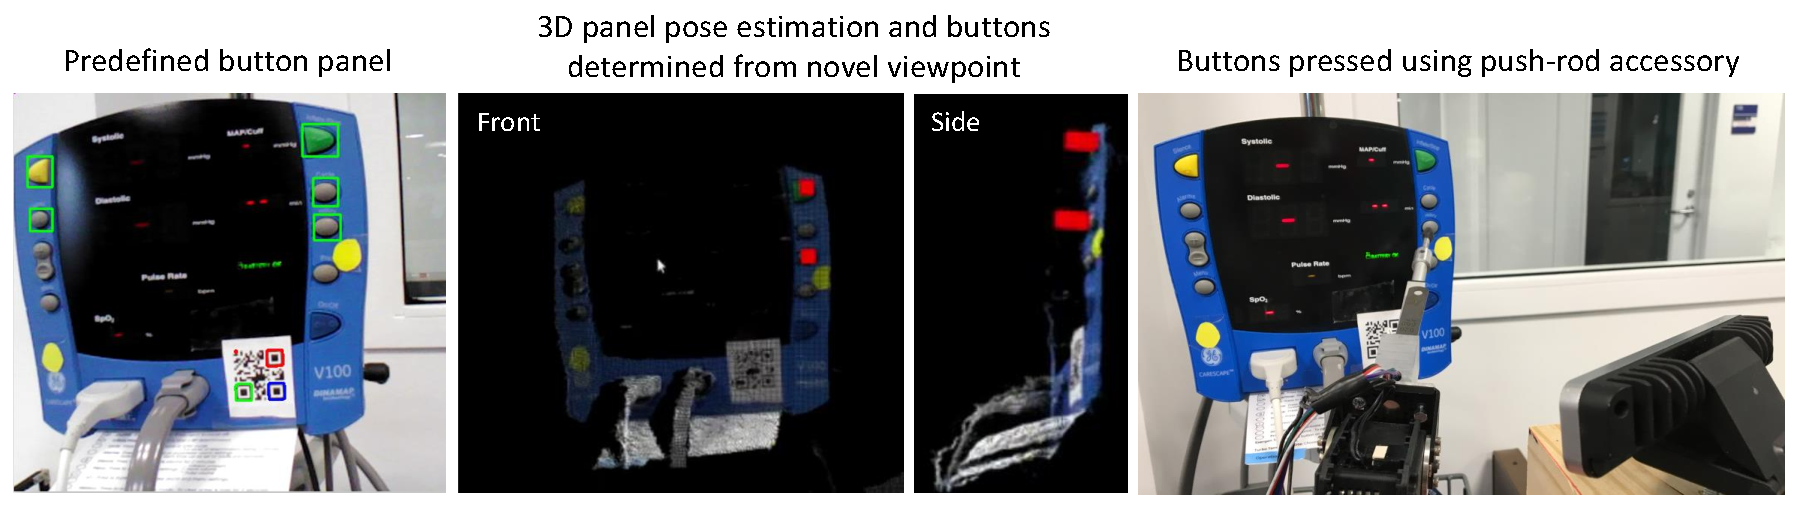
\includegraphics[width=0.9\textwidth]{fig/ButtonPressing.pdf}
\caption{Current work on a button pressing primitive skill. Left: A human prepares the environment by affixing a QR code, taking a single RGB+D image, and labeling button areas.  Middle and right: the system autonomously identifies button panels from novel viewpoints and presses the requested buttons using a precise pushing attachment.}
\label{fig:ButtonPressing}
\end{figure}

Current work is investigating strategies for autonomous button pressing.  We have already implemented a system for 3D mapping and identifying buttons in button panels (Figure~\ref{fig:ButtonPressing}) that requires a quick preparation of the clinical environment.  In the preparation phase, a 2\,cm$^2$ QR code is placed on the face of each button panel and a human gathers a clear picture and 3D scan of the button panel.  Then, the human labels the button panel and identifies and labels each button.  The segmented 3D scan, labels, and positions of each button are stored to a database.  This step takes approximately 1--3 minutes depending on the number of buttons on the panel, and can be performed with a laptop equipped with a 3D scanner or with the sensors on the robot.
%
For online detection, the robot is maneuvered close to the button panel, the QR code is detected by the robot's camera sensors and the robot moves into position to get a clear en-face view of the panel.  The 3D model of the panel is retrieved  from the database and registered to the RGB+D sensor data using the iterative closest points (ICP) algorithm.  Inverse kinematics is then used to press the button using the push-rod attachment of TRINA 1.0.  In preliminary tests, this method was able to operate 98.7\% of buttons and switches in a home and an office building~\cite{WangHauser2018}.
Once successfully integrated, button pressing will be decomposed into ``Localize Button'' and ``Operate Button'' primitive skills.

\paragraph{Pick-and-place.}  We will build on well-established techniques for autonomous grasping of objects on tabletops and placing them in collision-free locations, which will be useful for food tray preparation and waste disposal.   More advanced pick-and-place primitives may require identifying and separating objects in close contact (e.g., piles, stacks, against the edges of containers), transporting objects upright or with both hands, and manipulating deformable objects.

\paragraph{Surface cleaning.}  Discussions with nurses have also revealed that cleaning of bodily fluids is a frequently requested functionality of the robot.  We plan to enable the robot to clean a variety of surfaces like floors, tabletops, beds, medical equipment, and armrests via the primitive skills ``Prepare Cleaning Materials,'' ``Bulk Clean Area,'' ``Detail Clean Area,'' ``Dispose Cleaning Materials,'' and ``Clean Hands.'' Primitive areas will be defined as planar patches parameterized by location and shape, and cleaning will occur by moving the cleaning material along a fixed wiping pattern adapted to the size and location of the area.  More complex objects like beds and equipment will be defined as collections of multiple primitive areas.  If time permits, we will investigate vision algorithms for identifying soiled surfaces to clean more thoroughly.

\paragraph{Instrument placement against patient.} Instruments to collect vital signs should be placed against or near the patient in well-defined locations.  However, it takes a fair amount of training for human operators to determine where to position the robot's base and orient its appendages to reach those locations. The space near a bedridden patient is often cluttered, and for unresponsive or immobile patients the robot may need to also lift the patient's arm or move bed linens.  In this effort we plan to develop ``Navigate to Instrument Placement Location,'' ``Prepare Instrument Location,'' and ``Operate Instrument'' primitive skills.

\paragraph{Connect/disconnect tubing.} Nurses must frequently manipulate tubing for IVs, catheters, and suction containers to collect, replace, and dispose of fluids.  Attaching/detaching the connectors between tubes and containers (i.e., Luer-Lok) is a challenging task for teleoperation because it requires precise bimanual coordination of a combined twisting and pressing motion.  This primitive will use RGB-D sensing to identify the connector endpoints, connection status, and 3D reference coordinate system of each part.  Each part will be grasped by one of the end effectors, and then the appropriate twisting maneuver will be used.  To determine the necessary strength of twisting or pulling/pushing we will first attempt to use automated guarded moves with thresholds determined by connector type.  If this fails, we will fall back to a virtual fixture method~\cite{MOH2003} where the end effector paths are fixed, but progress along the path is guided by the human. 

\paragraph{Additional skill.} Once a basic suite of skills is generated, we will continue to consult with nurses to identify primitive skills that are necessary high-level clinical operation, high-priority, and/or repetitive.  Potential skills might include blood sample collection, opening sterile packaging, stripping bed linens, emptying waste containers, or pushing movable carts.  We will triage the development of recommended skills according to their clinical frequency and technical difficulty.

\paragraph{Capability testing.} Hardware upgrades to TRINA 2.0 will be evaluated using the same battery of clinical tasks in the nursing lab that were used to evaluate TRINA 1.0~\cite{LiTRINASystem2017}.  Trained nurse operators (n=12) will be asked to perform each task in direct teleoperation / shared control mode three times without direct line-of-sight (see Aim 3 for details on nurse recruitment). We will measure time and success rate. With the proposed upgrades, we hope to achieve at least 90\% of the identified nursing tasks (compared to 73\% in the prior version) and speed improvements of 30\% beyond the prior version.  Using the same protocol we will also evaluate novel tasks, such as wiping up a spill on the floor, which were physically impossible with TRINA 1.0 hardware.

Before inclusion in the library a primitive task will be evaluated for completeness of its specification and reliability levels.  Preconditions, postconditions, and error handling will be exhaustively unit-tested in the lab with a variety of objects and obstacle configurations, with at least 100 trials in total.  Our self-imposed quality requirements are that the preconditions, postconditions, and reported terminal status (success, failure, error) of the primitive to be correct at least 95\% of the time.



\subsubsection{Motion coordination assistance}
\textcolor{red}{TODO: Jane}

This task aims to study the motion coordination developed through various teleoperation interfaces that differ in motion mapping. It also investigates the teleoperated motion coordination performed under passive, active, and interactive perception. The teleoperated robot motion coordination are decomposed to low-level motion primitives and abstract the high-level motion coordination plan, of which the features are used to measure and compare the motion-perception coordination developed through different teleoperation interface, and under various perception mode. We further study the regularity and variability of the developed motion coordination across teleoperation interfaces, to reveal the adaption of human motor control to robot motion and perception capabilities.

In this task, we focus on the behavior of expert teleoperators. We assume with sufficient training, they have optimized the adaption of their motion coordination strategies to the motion and perception capabilities of the teleoperated robots. Through this task, we aims to:

\begin{itemize}

\item Develop a novel framework for evaluating the transparency of robot teleoperation interfaces. 

\item Identify the sets and frequent combinations of teleoperated robot motion primitives developed through different teleoepration interface. 

\item Construct high-level representation of the teleoperated motion coordinations using symbols for abstract states and option. 

\item Model the association of user's choice of camera views with the motion coordination plan to infer the motion-perception coordination strategy. 

\end{itemize}

Recently developed tele-nursing robots \cite{Li2017} are equipped with multiple manipulator arms, hands and mobile base. However, performing complex and dexterous motion coordination is still difficult even if the robots are under direct teleoperation of expert users. It is also hard for the teleoperator to perceive the remote environment and tasks through camera views, which affects the users' situation awareness, motion fluency and motion control accuracy. Previous research has compared teleoperation interface by their hardware capability and system configuration (e.g., field of view, camera viewpoints, depth perception, video frame rate, bandwidth limitations), time delay and control stability, sensory feedback channels (e.g., visual, audio, tactile display), motion control interfaces (e.g., voice, gesture, motion mapping control)~\cite{chen07, Zhu11,Luis14}, and augmented reality~\cite{Fritsche15,Garcia17,Peppoloni15,Brizzi18}. However, research so far hasn't systematically compared teleoepration interfaces by regularity and variability of the motion primitives and complexity of task plan in the teleoperated motion coordination.

Thus, we propose to learn from the teleoperated motion coordination demonstrated by expert users, to extract the robot's low-level motion primitives and high-level plan for nursing tasks that involves arm-hand coordination, bimanual coordination and loco-manipulation. We further compare the teleoperated motion coordination controlled through different user interfaces, and evaluate the interface usability in teleoperation. In addition to action motion coordination, we will also investigate the action and vision perception coordination, including when and how the teleoperator switch among multiple available camera views to facilitate the action being performed. Our proposed research contributes to the understanding of how human motor control adapt to the motion and perception capabilities of remote robotic surrogates. It also informs the design of human-robot teleoperation interface that can facilitate the learning of motion and perception mapping for novice users. 

\begin{wrapfigure}{r}{0.5\linewidth}
\centering
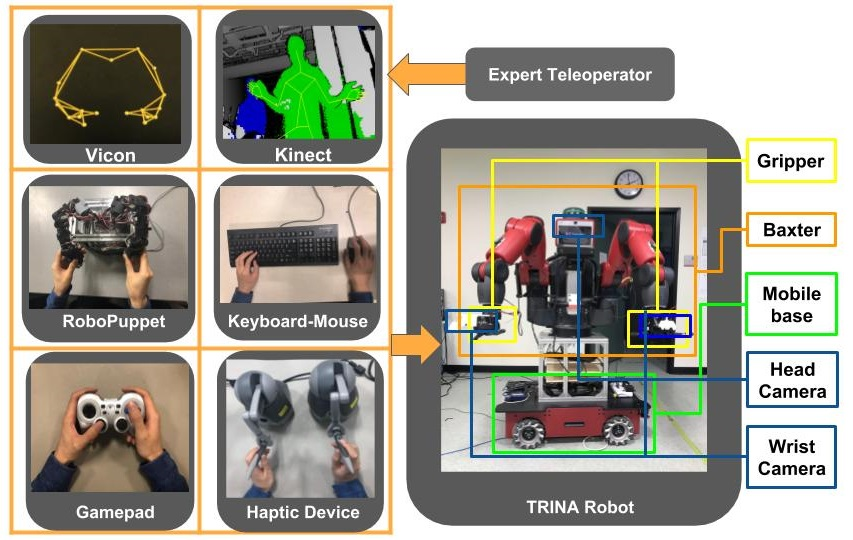
\includegraphics[width=0.5\textwidth]{fig//TeleInterface}
\caption{Teleoperation system software architecture}
\label{fig:TeleInterface}
\vspace{0.5ex}
\end{wrapfigure}


\paragraph{User study} Our user study aims to investigate how expert teleoperators control the motion coordination of a mobile humanoid robot through different teleoperation interfaces. We focus on the set of motion primitives developed through the usage of various robot control interfaces, and the task plan frequently used in arm-hand, bimanual and loco-manipulation coordination. Our experiment platform TRINA has a humanoid robot torso (Rethink Robotics Baxter), an omnidirectional mobile base (HStar AMP-I) and two three-fingered grippers (Righthand Robotics Reflex grippers)~\cite{Li2017}. Shown in~\fig{fig:TeleInterface}, our preliminary work has setup six input interfaces to control the motion of humanoid robot and its mobile base, including (1) keyboard and mouse, (2) gamepad, (3) Geomagic touch haptic devices, (4) RoboPuppet~\cite{}, and motion mapping from (5) Vicon motion capture system and (6) Kinect v2 camera. The platform also enables a teleoperator to use voice control to switch camera views, from the RGB+D cameras attached to the left and right hands, mounted on robot head, and from a standalone camera that look at the robot and workspace. 

Our user study will train subjects to be fluent in the teleoperation a mobile humanoid robot and perform teleoperated motion coordination tasks shown in~\fig{NursingTask}. We will record synchronized teleoperated robot motion, control interface input and interface visual display. We segment the collected data to extract motion primitives from the motion robot hand, arm and mobile bases, and coupled them if the motions are performed simultaneously. In addition, we also extract information for motion-perception coordination. We associate the camera view being used with the motion being performed. We also record task performance including task completion time, collisions with unwanted objects, and success rate over repetitive trials. 

\paragraph{Comparing motion primitives and task plan across teleoperation interfaces}


\paragraph{Inferring high-level motion coordination strategies to inform task automation}
The design of intelligent teleoperation interface poses the fundamental question of \textit{what is the appropriate task division between human and robot in shared-autonomous control}. Indeed, the control effort-sharing between robot automation and direct human control can refer to how human motor system regulate the controlled and uncontrolled manifolds. Take reaching-to-grasp motion for instance, as human focusing on control hand position and orientation, the arm posture (i.e., how to pose the elbow) is automatically handled. In bimanual coordination, human focuses more on the control of dominant hand, while dominant hand follows naturally and accordingly. 

In this study, we aim to examine the high-level motion coordination strategy for the coordination of macro-micro structures (e.g., arm-hand, based-arm), dominant/non-dominant arms, and action-perception arms. We hypothesis that given manipulation as the primary task, the adjustment of the mobiles base, non-dominant/perception arm and the action arm posture aims to (1) maximizing the action arm's manipulability and reachability to the candidate objects in workspace, (2) maintaining the stereoscopic visibility of the object being manipulated, and minimizing the amount of large (robot) motion. To evaluate this hypothesis, we apply inverse reinforcement learning to the high-level motion coordination plans modeled as semi-markov decision processes. We shape a reward function based on the considerations in our hypothesis and use the inferred weighting coefficients to evaluate their validity.  

\subsubsection{Adaptive task scheduling}
\textcolor{red}{TODO: Missy}

To address current challenges in scheduling and optimization of collaborative human-autonomy environments, we propose the development of the Collaborative Human-Autonomy Replanner for Medical Systems (CHARMS). Through models of the interdependencies between agents and impacts of agent failures, CHARMS will provide ``smart'' decision support for schedulers to identify and adapt to dynamic scheduling challenges in healtchare environments. Additionally, CHARMS will track ergonomic risk for human workers and failure risk for robots, enabling schedulers to manage both long and short term safety though proactive scheduling. 

CHARMS is a decision support tool that allows a supervisor to understand the impact of an agent (human or robot) ``failure'' across different work environments. CHARMS aids the supervisor in developing a contingency plan to mitigate production impact while maintaining a safe work environment. The development of CHARMS will utilize human-centered design, drawing upon interviews, demonstrations, and reviews with representative nursing personnel. CHARMS will be developed and tested in a mock hospital setting.

To date, there are no products available on the commercial product that can perform the full set of functions proposed for CHARMS. There are a variety of available industrial scheduling software packages that can assist with process sequencing and shift scheduling (e.g. Optessa, TACTIC, Lean Factory Management), but these are focused on human work scheduling and to our knowledge, none of these account for collaborative human-autonomy work architectures. 

Beyond considerations of ergonomic risk, from a dynamic rescheduling perspective unstructured collaborative environments provide greater flexibility in that both robots and humans can potentially act as a replacement for an absent human or malfunctioning robot. However, in these environments there are additional considerations for the certification of the agents in each of the tasks as well as the impacts of varying task completion efficiency on the productivity as a whole. To address related questions and provide a tool that incorporates a deep understanding of types of collaborative architectures and their resilience to perturbations in scheduling, the proposed work includes these primary elements:

\begin{enumerate}
    \item Determining a core set of design requirements and principles as well as detailed test and evaluation strategies in the development of a smart scheduling system for collaborative human-robot teaming in a manufacturing setting. This will include how a dynamic rescheduling system should be designed to capture the capabilities and limitations of both. We especially want to focus on the balance of work between robots and humans in order to minimize the ergonomic risk of human repetitive stress injuries.
    \item Creating an implementation of this smart scheduling systems with an emphasis on human-systems design principles and advanced optimization algorithms that focus on satisficing in the presence of uncertainty. In addition, these algorithms will be able to learn from the human coach to better tailor future solution recommendations.
    \item Conducting integrated testing utilizing actual robotic agents in a mock manufacturing environment.
    \item	Determining how the results from the design and tests in this representative environment can be extended to other healthcare settings. 
\end{enumerate}

The integration of robotic agents into CHARMS will focus on developing a set of representations of clinical workflow under collaborative human-autonomy environments. These representations will capture the temporal and physical interdependencies between tasks and workers (for both divisional and integrated collaborative human-autonomy environments). Additionally, CHARMS will be customizable to account for certifications, programming/re-programming restrictions, etc. that separate structured and unstructured environments and utilize these constraints in the generation of new replanning solutions.

Proposed functionalities based on initial discussions include:
\begin{itemize}
\item Characterization of a skill, rule, and knowledge-based cognitive reasoning taxonomy that will be needed to classify the basic requirements of collaborative tasks, both structured and unstructured (Rasmussen, 1983; Cummings M. , 2014).
\item Ability to request automated replanning and recommendations through optimization algorithms
\item Provide scheduling recommendations that account for the nature of the work environment (structured vs. unstructured), ergonomic risk, potential reliability issues, and that highlight potential safety compromises.
\item Ability for a supervisor to investigate changes to the schedule and coach the algorithms if needed
\item Provide alerts upon a change (both descriptive and predictive) in status of one of the robotic or human agents (e.g. malfunction or unexpected absence)
Our prior research on design of future systems and interfaces has included the development of the Hybrid Cognitive Task Analysis (hCTA) (Nehme, Scott, Cummings, \& Furusho, 2006). The hCTA methodology provides a principled approach to cognitive task and work analysis for systems that do not yet exist, such as the proposed integrated collaborative human-autonomy work environment. 
\end{itemize}

Specific goals for this task include: 
\begin{itemize}
    \item As a system designed to augment human decision-making capabilities, the design and implementation of CHARMS must consider the human as an integral part of the system and follow appropriate principles to maximize the human-machine performance. 
    \item The integration of collaborative human-autonomy environments as part of the CHARMS system must draw upon expertise in robotic systems, and these skills will be critical in the creation of a testbed for evaluating the system performance
    \item CHARMS will integrate with the onboard health and status monitoring of the robotic agents in order to provide the user with current information and alerts in case of a malfunction. These sources of information would be used as part of status visualizations for human decision makers in a decision support environment as well as inform the scheduling optimization algorithms. 
    \item The backbone of the CHARMS system focuses on replanning in uncertain environments, which will require careful consideration of approaches for schedule optimization or ``satisficing.''
    \item To provide a ``risk-aware'' scheduling system, CHARMS requires tracking and modeling of human ergonomic risk as well as robot reliability and prediction of necessary maintenance.
\end{itemize}

The evaluation of this task will utilize Duke Robotics facilities and personnel to test the implementation in a simulated tele-nursing environment with a robotic agent. This phase of lab testing will focus on the integration of the CHARMS system with the robotic and human agents and improve the understanding of scheduling in structured and unstructured environments. An initial version of the CHARMS software will be developed and installed on a computer system integrated with a set of robotic agents. This integration will include bi-directional communications allowing the central system to receive health and status information from the agents (such as a robotic malfunction) as well as distribute general tasking commands to the robotic agents. The development of this testing environment and the robotic worker actions will leverage prior work on validated human-robot interaction metrics (Cummings \& Donmez, 2013; Steinfeld, et al., 2006; Goodrich \& Schultz, 2007). Testing of the system will focus on a variety of conditions in the simulated environment to ensure proper functionality of the CHARMS system, including:
\begin{itemize}
    \item Identification of a malfunction of a robot worker
    \item Supervisor input of human worker absence or incapacity.
    \item Rescheduling of tasks and agents due to the unavailability of an agent, under several architectures:
    \begin{itemize}
        \item Divisional and structured: Tasks performed in series, only allow human replacements of human workers, requires specified maintenance distribution time to repair for robotic agents.
        \item Divisional and unstructured: Tasks performed in series, allow both human and robotic replacements for robotic workers, only human replacements for human workers
        \item Integrated and structured: Tasks performed simultaneously, only allow human replacements of human workers, requires specified maintenance distribution time to repair for robotic workers
        \item Integrated and unstructured: Tasks performed simultaneously, allow both human and robotic replacements for robotic workers, only human replacements for human workers
    \end{itemize}
\end{itemize}

%-------------------------------------------------------------------------
\subsection{Specific Aim 2: Model the socioeconomic impact of healthcare robots}\label{sec:plan-task2}
%-------------------------------------------------------------------------
\subsubsection{Economic and labor market analysis}
\textcolor{red}{TODO: Alex}

\subsubsection{Attitudes of personnel to robotics}
\textcolor{red}{TODO: Missy, Jeanine, or Ryan?}

\subsubsection{Bias and disparate impact analysis}
\textcolor{red}{TODO: Jeanine}

%-------------------------------------------------------------------------
\subsection{Aim 3: Model the interaction between autonomy and impact}\label{sec:plan-task3}
%-------------------------------------------------------------------------

\subsubsection{Design of the human-autonomy interface}
\textcolor{red}{TODO: Missy}

\subsubsection{Effects of interface and autonomy on bias}
\textcolor{red}{TODO: Jeanine}

\subsubsection{Formulate best practices}
This task aims to evaluate motor skill progression and recovery with the assistance of human-autonomy interface for nursing, surgical and rehabilitation robots. We conduct user studies to investigate the evolution of motion coordination (e.g., motion primitives and task plans), motion economy, and demand of conscious attention as the motor skills of the robot users develops from novice (paretic) to expert (healthy) level. We hypothesize that , they have optimized the adaption of their motion coordination strategies to the motion and perception capabilities of the teleoperated robots. Through this task, we aims to:





\subsection{Milestones and Timeline}


\input{004BroaderImpact.tex}
\section*{Results from Prior NSF Support}

Dr. Hauser has been the PI of five NSF grants (RI-1218534, \$381,168, 8/2012–7/2015), (CAREER-1253553, \$481,151, 8/2013–7/2018), (SCH-1343940, \$686,411, 3/2014–2/2017), (IIS-1513221, \$73,025. 12/2014-11/2015) (NRI-1527826, \$472,712, 10/2015-9/2018). The CAREER and IIS RAPID grants, ``Cooperative Motion Planning for Human-Operated Robots'' and ``RAPID: Tele-Nursing Robots for Remote Treatment of Ebola Patients'' are the most closely related. \\
{\bf Intellectual Merit:} These grants studied methods for introducing greater robot intelligence in teleoperation systems, including the use of collision checking, motion planning, and grasp planning under the direction of human operators. Most results so far are on algorithms for satisfying the competing demands of both responsive and optimized motions. They have yielded 7 published publications so far (see references 14, 28, 29, 30, 40, 41, 42). \\
{\bf Broader Impacts:} A workshop on Algorithmic Human-Robot Interaction (AHRI) at the Human-Robot Interaction Conference and a AAAI Fall Symposium on Artificial Intelligence in Human-Robot Interaction (AI-HRI) were organized as part of the CAREER grant. One undergraduate REU student was funded for each summer of the CAREER grant, including one that resulted in a published paper (Eilering et al 2014), and a female student completed her PhD in Computer Science under support from this grant.  Five undergraduate independent studies were supervised as a part of the RAPID grant, which also contributed to enhancing institutional infrastructure for robotics research by providing hardware and software components for a teleoperated mobile manipulator.


Dr. Cummings served as PI of an NSF EAGER: Modeling Intent Communication Pathways for Human-Autonomous System Collaboration (\#1548417, \$299,990, 09/01/2015-08/31/2017).  The focus of this effort is to develop models of the signals, signs and symbols that inform skill, rule, and knowledge-based responses for both humans and autonomous systems attempting to cope with uncertainty. 
Summary of Results: This effort only just started so there are no empirical results as of yet. We are currently developing an experimental protocol to address intent communications in driverless car settings that include pedestrians. \textcolor{red}{TODO: update with new pubs}.  \\
{\bf Intellectual Merit:} This project determined how elements of the environment, the computation systems of robots, and unique traits of humans (including attention management) can be modeled to represent intent communication pathways that need to be instantiated in the system or the world around the system.\\
{\bf Broader Impact:} includes broader social impact in driverless car and manufacturing settings, and  there is significant potential to impact these rapidly developing domains.

Dr. Shaw (Duke), Dr. Li (WPI) have not received prior NSF support.



\pagebreak
\setcounter{page}{1}
\setcounter{section}{0}

\section{Collaboration Plan}

\subsection{Summary}

Co-PIs from both engineering and the social sciences are co-located at each of the three partnering institutions (Duke University, Worcester Polytechnic Institute, and UCLA).  This will permit more frequent local activities to be conducted between larger-scale collaborative efforts across institutions.

The team at Duke (Hauser, Cummings, Shaw) will concentrate on the tele-nursing application and continues an existing collaboration between Duke’s Pratt School of Engineering and the School of Nursing. More broadly, the Duke team will contribute toward expertise in semi-autonomous decision making and human factors. The team will benefit from the relatively close proximity between the School of Engineering and the School of Nursing, and the TRINA robot has been transported twice already to the School of Nursing’s Simulation Lab to perform extended experiments.

The team at WPI (Li, Skorinko, Smith) will focus on the in-home assistance and rehabilitation application and will contribute to expertise in human motor control, bias and pro-social behavior.  WPI team will take the lead to study social-economical impacts of robot usage in healthcare, and will focus on bio-inspired robot control and robot-assisted motor learning.  Both Duke and WPI have a shared TRINA mobile manipulator platform which will facilitate software and infrastructure sharing. WPI and UCLA are collaboratively developing a home-based upper limb rehabilitation system and will share the platform for this research collaboration. 

The team at UCLA (Rosen, ...) will focus on telesurgery and rehabilitation applications, and will contribute to expertise in development, autonomous control and clinical application of large surgical and rehabilitation robot systems. The UCLA team will take the lead in development and clinical evaluation of cognitive augmentation technologies for assisting decision-making and skill evaluation in surgery and rehabilitation. The UCLA team will collaborate with WPI team on development and evaluation of home-based stroke rehabilitation system. 

\subsection{Meetings, Site Visits, and Student Exchange}

In-person meetings will be held between all of the Co-PIs and students at individual institutions at least monthly, and study personnel on individual Tasks will meet more frequently on an as-needed basis. 

Site visits will be held thrice yearly to help coordinate project goals and activities between institutions. These one-day workshops will involve discussion of past findings, current plans, and brainstorming. The budget for each institution includes travel for two personnel to attend these workshops, twice yearly. 

Activities in Aims 1 and 2 will be pursued largely by each institution in parallel, and using the medical domain in which the institution has greatest expertise. Coordination across institutions will be more intense in Aim 3 (Year 3), and we plan to host student exchanges during the summers or academic year in order to accomplish project goals.

\subsection{Specific roles of the Investigators}

PI Hauser (Duke) provides expertise in robotics and artificial intelligence, and he will coordinate project activities and lead the development of Task 1.1 (Automation of routine tasks) on the tele-nursing application.  He will also collaborate closely with Co-PI Cummings and Skorinko on designing and evaluating the human-autonomy interface.

Co-PI Cummings (Duke) provides expertise in human factors and human-robot interaction, and will led the development of Task 1.3 (Adaptive task scheduling) and 3.1 (Design of the human-autonomy interface).

Co-PI Li (WPI) provides expertise in human motor control and robotics, and will lead the development of Task 1.2 (Motion coordination assistance) on the in-home care and rehabilitation robotics applications.  She will also coordinate closely with Co-PI Skorinko on Task 2.3 during the robot evaluation portion of the study.

Co-PI Rosen (UCLA) provides expertise in robotic surgery and rehabilitation, and he will conduct Task 1.1 (Automation of routine tasks) in the context of the tele-surgery application, and will collaborate closely with Co-PI Li on Task 1.2 as applied to rehabilitation robotics.  

Co-PI Shaw (Duke) provides expertise in nursing and e-Health, and will lead the nursing component of Task 2.2 (Attitudes of personnel to robotics).

Co-PI Skorinko (WPI) provides expertise in psychology and gender bias, and will...

Co-PI Smith (WPI) provides expertise in economics, and will...

\pagebreak
\setcounter{page}{1}
\setcounter{section}{0}

\pagebreak
\setcounter{page}{1}
\setcounter{section}{0}

\pagebreak
\setcounter{page}{1}
\setcounter{section}{0}


\bibliographystyle{IEEEtran}
\bibliography{./ZhiLi_ref,hauser_refs}

\end{document}
